\subsection{Отримані результати}
Оцінка якості роботу розроленого методу та його порівняння відбувалась на декількох датасетах сформованих за методологією наведеною вище. У якості наборів еталонних зображень висптупили PEXELS300 та BSD500. Запустивши автоматизоване тестування у розробленому прогрманому комплексі ми отримаємо наструпні наведені результати для різних коефіцієнтів мастабування та наборів даних:

\begin{figure}[htbp]
	\centering
	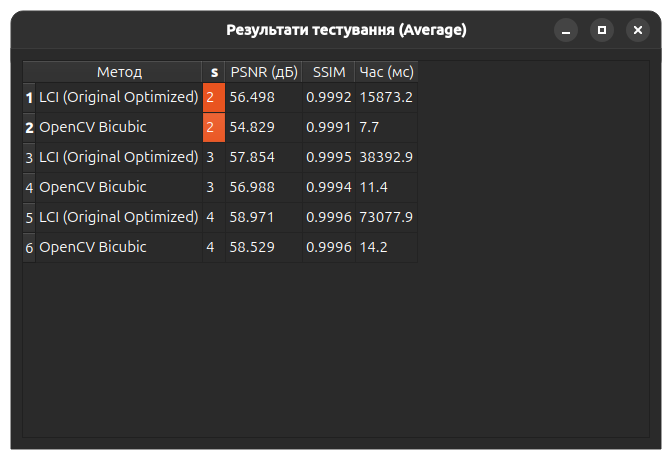
\includegraphics[width=0.9\textwidth]{figures/PexelsLCIvsBIC.png}
	\caption{Результати роботи барицентричного оптимізованого проти OpenCV bicubic у напрямку зменшення (PEXELS300)}
\end{figure}

\newpage

\begin{figure}[htbp]
	\centering
	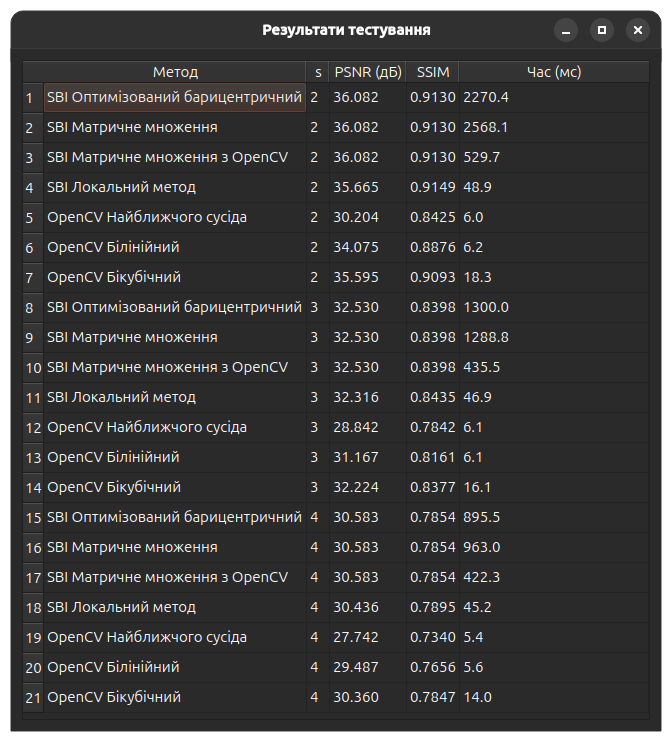
\includegraphics[width=0.9\textwidth]{figures/PEXELS_Up_Scale.png}
	\caption{Результати роботи барицентричного оптимізованого та методів OpenCV у напрямку збільшення (PEXELS300)}
\end{figure}

\newpage
\begin{figure}[htbp]
	\centering
	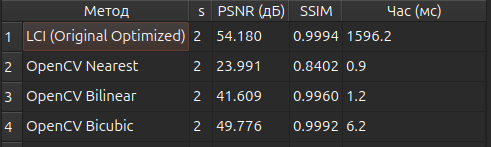
\includegraphics[width=0.7\textwidth]{figures/bsd/2}
	\caption{Результати роботи барицентричного оптимізованого та методів у напрямку зменшення [s=2] (BSD500)}
\end{figure}

\begin{figure}[htbp]
	\centering
	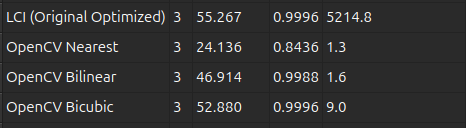
\includegraphics[width=0.7\textwidth]{figures/bsd/3}
	\caption{Результати роботи барицентричного оптимізованого та методів у напрямку зменшення [s=3] (BSD500)}
\end{figure}

\begin{figure}[htbp]
	\centering
	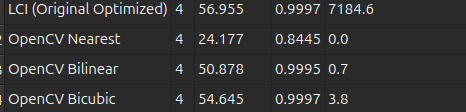
\includegraphics[width=0.7\textwidth]{figures/bsd/4}
	\caption{Результати роботи барицентричного оптимізованого та методів у напрямку зменшення [s=4] (BSD500)}
\end{figure}

\newpage
\begin{figure}[htbp]
	\centering
	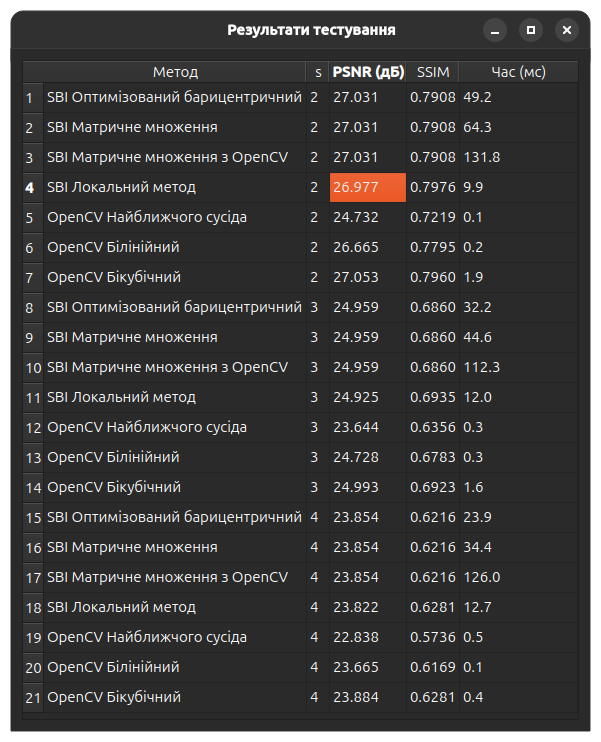
\includegraphics[width=0.9\textwidth]{figures/BSD_Up_Scale.png}
	\caption{Результати роботи барицентричного оптимізованого та методів OpenCV у напрямку збільшення (BSD500)}
\end{figure}
